%
% polylog.tex
%
% (c) 2026 Prof Dr Andreas müller
%
\begin{figure}
\centering
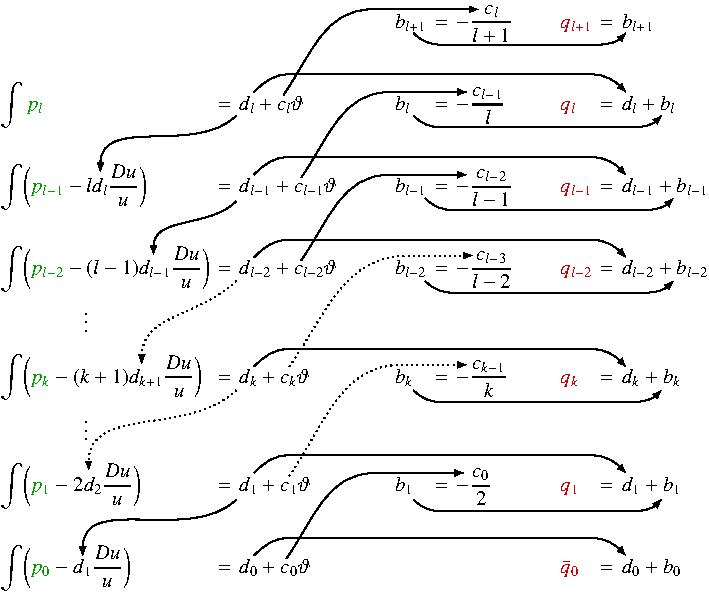
\includegraphics{chapters/070-intalg/images/polylog.pdf}
\caption{Gang der Rechnung für den polynomiellen Teil im Fall einer
logarithmischen Erweiterung.
Aus den bekannten Koeffizienten $p_k\in F$ wird zunächst der Integrand
gebildet, wozu $d_{k-1}$ aus dem vorangegangenen Schritt benötigt wird.
Die Stammfunktion liefert $d_k$ und die Konstante $c_k$, mit der sich
die Integrationskonstaten $b_{k-1}$ im vorangegangenen Schritt
festlegen lässt.
\label{buch:intalg:risch:logarithmisch:fig:polylog}}
\end{figure}
